\documentclass[twocolumn,superscriptaddress,showpacs,preprintnumbers,amsmath,amssymb,prl]{revtex4-1}
\usepackage{siunitx}
\usepackage{tikz}
\usetikzlibrary{arrows,shapes,backgrounds, calc, positioning, topaths,chains, intersections, decorations.markings, shapes.geometric, matrix,patterns,mindmap,fit}
%\usetikzlibrary{positioning, patterns,topaths,chains,matrix}

\usepackage{pgfplots}
\usepackage{pgfplotstable}
\pgfplotsset{compat=1.9}
\usepgfplotslibrary{groupplots}
\usepgfplotslibrary{external}
\tikzsetexternalprefix{fig_long/}
\tikzexternalize
\tikzset{external/force remake}

\begin{document}
\pgfplotscreateplotcyclelist{earthy}{%
red!40!black,
red!60!black,
red!80!black,
red,
red!80!yellow,
red!60!yellow,
red!40!yellow,
}
\tikzsetnextfilename{structure_finale}
%\begin{figure}
\begin{tikzpicture}[every node/.style={inner sep=0}]
\matrix[matrix of nodes, row sep=3pt, column sep=0] (m){
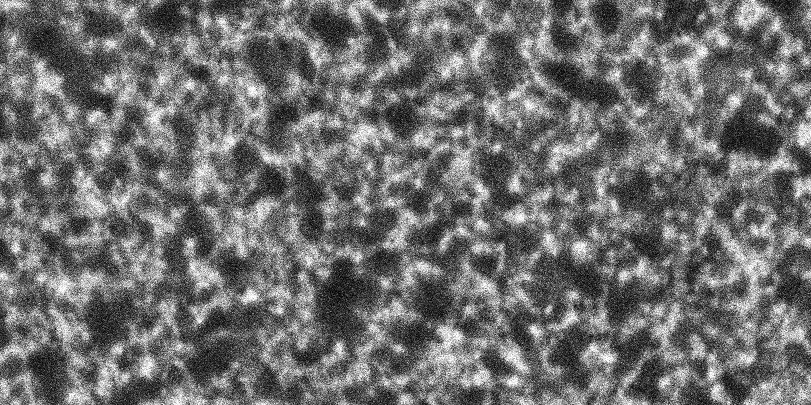
\includegraphics[width=\columnwidth]{ech17_x63_time699_crop.jpg}\\
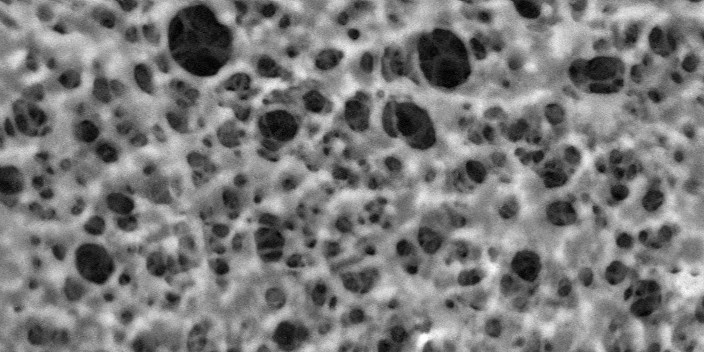
\includegraphics[width=\columnwidth]{ESEM_cas4_GDL1-17_crop.jpg}\\
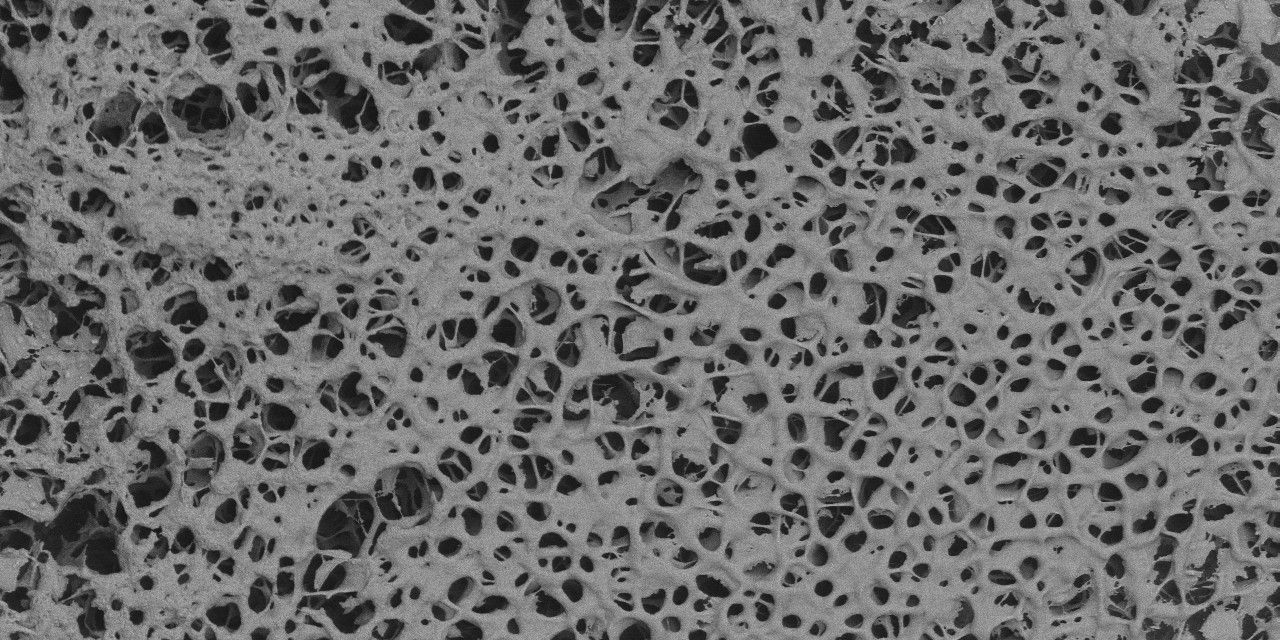
\includegraphics[width=\columnwidth]{SEM_cas4_gdl1_22_crop.jpg}\\
};
\foreach \i in {1,2,3}
\draw[ultra thick, white] (m-\i-1.south east) ++(-1em,1em) -- +(-0.25\columnwidth,0);
\end{tikzpicture}
\caption{Final structure of caseinate 4\%, GDL 4\% gels, observed by fluorescent confocal micoscopy, environmental SEM and cryo SEM.}
\end{figure}
\tikzsetnextfilename{prise_cas4}
\begin{figure}
\begin{tikzpicture}
\begin{axis}[
	name=unscaled,
	height=0.5\columnwidth,
	width=\columnwidth-1em,
	xlabel={time (h)}, ylabel={$G^\prime$ (\si{\pascal})},
	cycle list name=earthy,
	no marks,
	xmin=0, xmax=20,ymin=0,
	]
	\begin{scope}[every node/.style={anchor=base west, inner xsep=0,font=\footnotesize}]
	\addplot table[x expr={\thisrowno{0}/3600}]{cas4_GDL1_Y265.prise} node {1\%};
	\addplot table[x expr={\thisrowno{0}/3600}]{cas4_GDL1.25_Y277.prise} node {1.25\%};
	\addplot table[x expr={\thisrowno{0}/3600}]{cas4_GDL1.5_Y275.prise} node {1.5\%};
	\addplot table[x expr={\thisrowno{0}/3600}]{cas4_GDL2_Y268.prise} node[yshift=0.1em] {2\%};
	\addplot table[x expr={\thisrowno{0}/3600}]{cas4_GDL3_Y270.prise} node[yshift=-0.1em] {3\%};
	\addplot table[x expr={\thisrowno{0}/3600}]{cas4_GDL4_Y271.prise} node[yshift=-0.6em] {4\%};
	\end{scope}
\end{axis}
\begin{loglogaxis}[
	name=scaled,
	anchor=north west, 
	at=(unscaled.below south west), 
	width=0.5\columnwidth-0.5em,
	height=0.375\columnwidth,
	cycle list name=earthy,
	no marks,
	xmin=1e-3, xmax=1e2, ymin=1e-3, ymax=2,
	xlabel=$(t-t_i)/(t_m-t_i)$, 
	ylabel=$G^\prime/G^\prime_m$ ,
]
	\addplot table[x expr={(\thisrowno{0}-7758)/(28840-7758)}, y expr={\thisrowno{1}/883}]{cas4_GDL1_Y265.prise};
	\addplot table[x expr={(\thisrowno{0}-5179)/(14240-5179)}, y expr={\thisrowno{1}/788}]{cas4_GDL1.25_Y277.prise};
	\addplot table[x expr={(\thisrowno{0}-3839)/(9640-3839)}, y expr={\thisrowno{1}/726}]{cas4_GDL1.5_Y275.prise};
	\addplot table[x expr={(\thisrowno{0}-2519)/(5720-2519)}, y expr={\thisrowno{1}/665}]{cas4_GDL2_Y268.prise};
	\addplot table[x expr={(\thisrowno{0}-1369)/(3120-1369)}, y expr={\thisrowno{1}/589}]{cas4_GDL3_Y270.prise};
	\addplot table[x expr={(\thisrowno{0}-758)/(1890-758)}, y expr={\thisrowno{1}/500}]{cas4_GDL4_Y271.prise};
\end{loglogaxis}
\begin{axis}[
	anchor=north east, 
	name=desc,
	at={(unscaled.below south east)}, 
	width=0.5\columnwidth-0.5em,
	height=0.375\columnwidth,
	cycle list name=earthy,
	no marks,
	xmode=log, xmin=1e-1, xmax=1e2,
	ymin=0, ymax=1.1,
	xlabel=$(t-t_m)/(t_m-t_i)$, 
	ylabel=$\displaystyle\frac{G^\prime-G^\prime_\infty}{G^\prime_m-G^\prime_\infty}$ ,
	%ylabel=$(G^\prime-G^\prime_\infty)/(G^\prime_m-G^\prime_\infty)$ ,
	]
	\addplot table[x expr={(\thisrowno{0}-28840)/(28840-7758)}, y expr={(\thisrowno{1}-616)/(883-616}]{cas4_GDL1_Y265.prise};
	\addplot table[x expr={(\thisrowno{0}-14240)/(14240-5179)}, y expr={(\thisrowno{1}-325)/(788-325}]{cas4_GDL1.25_Y277.prise};
	\addplot table[x expr={(\thisrowno{0}-9640)/(9640-3839)}, y expr={(\thisrowno{1}-200)/(726-200}]{cas4_GDL1.5_Y275.prise};
	\addplot table[x expr={(\thisrowno{0}-5720)/(5720-2519)}, y expr={(\thisrowno{1}-145)/(665-145}]{cas4_GDL2_Y268.prise};
	\addplot table[x expr={(\thisrowno{0}-3120)/(3120-1369)}, y expr={(\thisrowno{1}-103)/(589-103}]{cas4_GDL3_Y270.prise};
	\addplot table[x expr={(\thisrowno{0}-1890)/(1890-758)}, y expr={(\thisrowno{1}-75)/(500-75}]{cas4_GDL4_Y271.prise};
\end{axis}
\begin{scope}[every node/.style={anchor=south east, text height=0.8em, text depth=0.2em, font=\Large\bfseries}]
\node at (unscaled.south east) {a};
\node at (scaled.south east) {b};
\node at (desc.south east) {c};
\end{scope}
\end{tikzpicture}
\end{figure}
%\tikzsetnextfilename{prise_cas4_scaling_factors}
%\begin{figure}
\begin{tikzpicture}
\begin{groupplot}[
	group style={
			group name=g, group size=1 by 2,
		},
	width=\columnwidth,
	height=0.5\columnwidth,
	xlabel={GDL (\%)},
	xmin=0, xmax=4.5,
	]
\nextgroupplot[ylabel={$G^\prime$ (\si{\pascal})}, ymin=0,]
	\addplot[red!40!black,, mark=*] table{scaling_factors_prise.txt} node[above] {$G^\prime_m$};
	\addplot[red!80!yellow,, mark=o] table[y index=2]{scaling_factors_prise.txt}  node[above] {$G^\prime_\infty$};
\nextgroupplot[ylabel={$t_m-t_i$ (\si{\second})},ymode=log,ymin=5e2,ymax=5e4]
	\addplot[red, mark=star] table[y expr=\thisrowno{3}-\thisrowno{4}]{scaling_factors_prise.txt};
	\addplot[red!40!black, mark=*] table[y index=3]{scaling_factors_prise.txt } node[right] {$t_m$};
	\addplot[red!40!yellow, mark=o] table[y index=4]{scaling_factors_prise.txt} node[right] {$t_i$};
\end{groupplot}
\end{tikzpicture}
\end{figure}
\end{document}